\section{Metadata Performance}

\begin{figure}[htb]
\centering
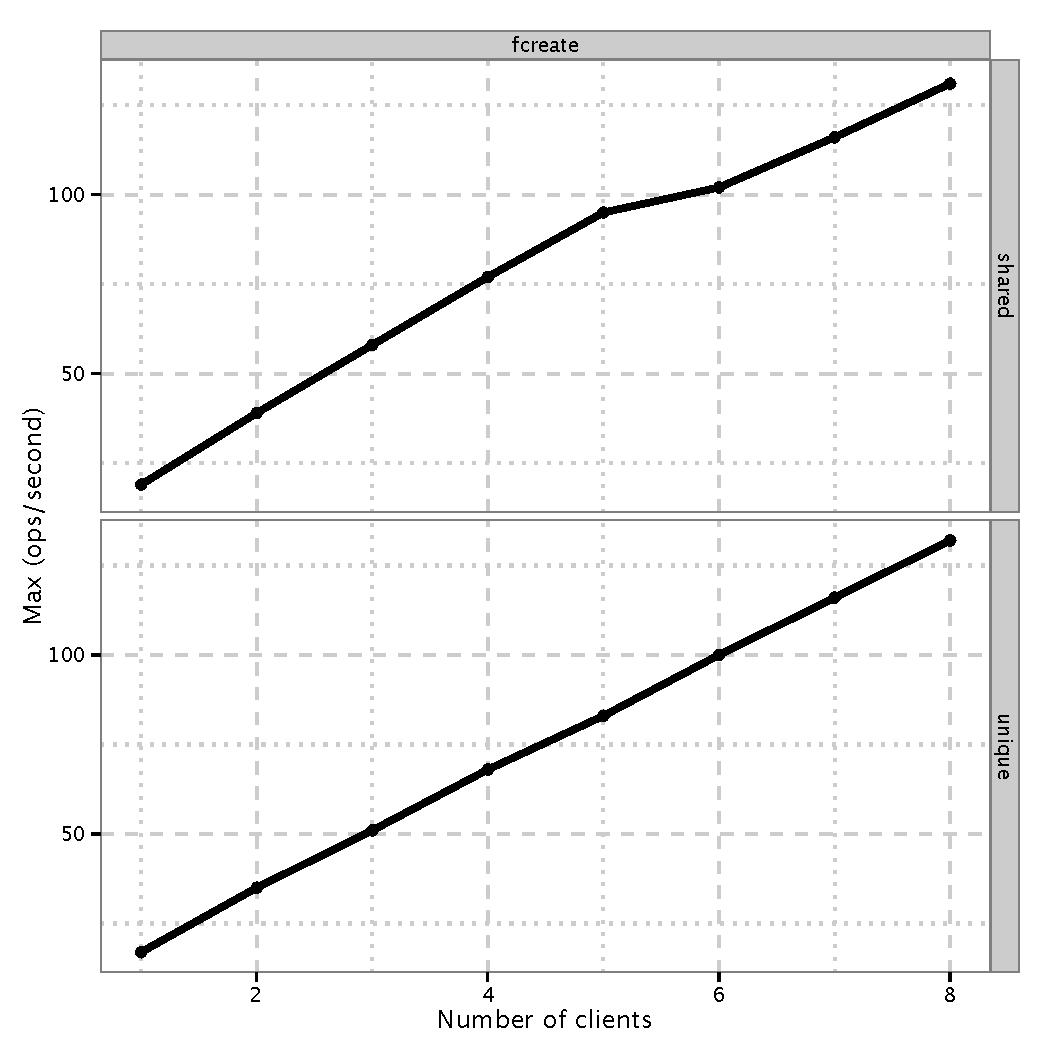
\includegraphics[width=3in]{data/mdtest-fcreate}
\caption{File creation vs.  number of clients}
\label{fig:mdtest-fcreate}
\end{figure}

\begin{figure}[htb]
\centering
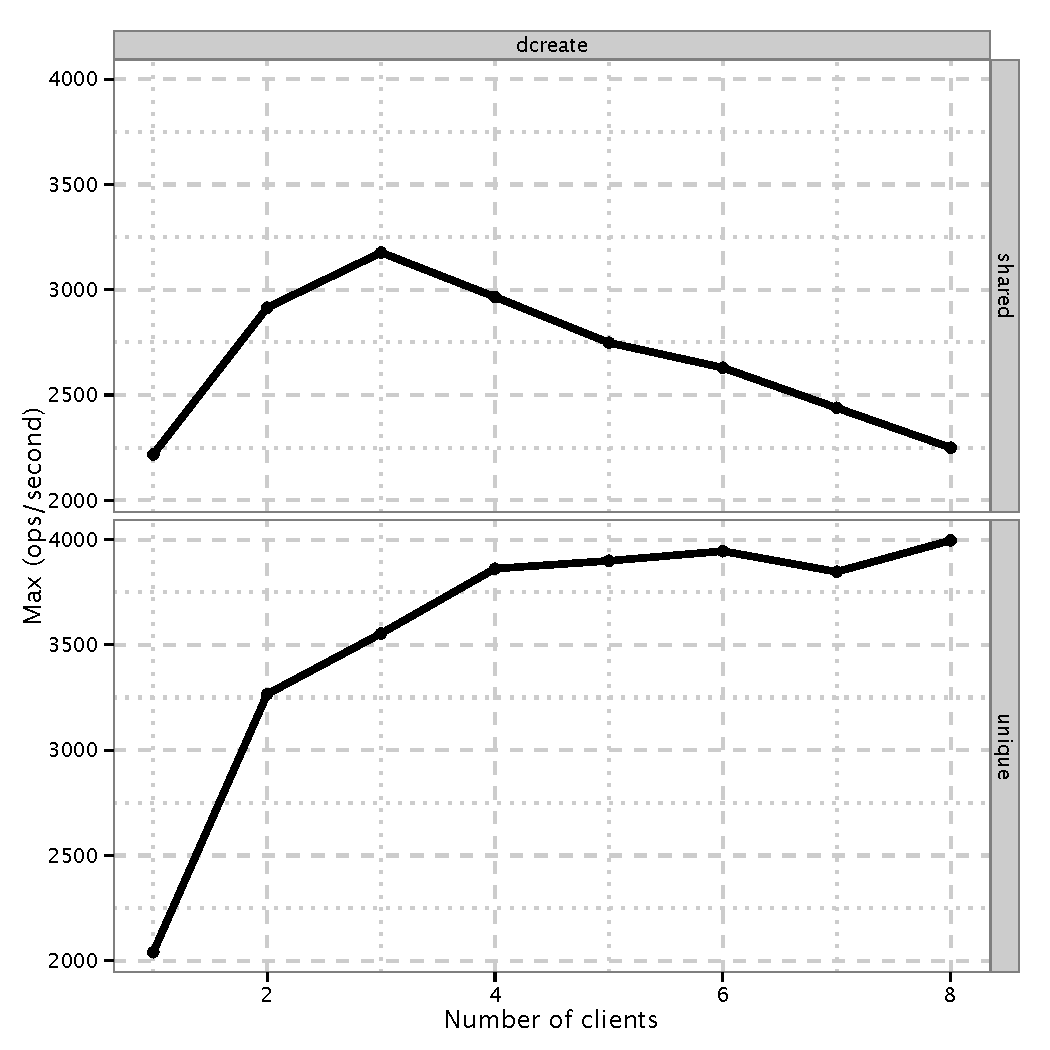
\includegraphics[width=3in]{data/mdtest-dcreate}
\caption{Directory creation vs. number of clients}
\label{fig:mdtest-dcreate}
\end{figure}


In our particular setup, we only had one metadata server (MDS) configured.
Therefore, this is not a scalability test on the performance of Ceph clustered
MDS, which would have been very interesting.  Instead, we focus on a single MDS
performance and exercise it with up to 8 clients to observe the single MDS
performance scaling. We used mdtest as our benchmark tool. Mdtest parameters
used for this test are:

\begin{itemize}
\item \verb!-w 1048576 -y!: for each created file, we write 1 MB data and
perform a sync operation.  This is a more realistic use case scenario than just
open, close and removal sequence of metadata operations.

\item \verb!-n 1000!: Per client file \textit{and} directory workload. For eight
clients, the total number of files and directories in the workload is 8,000. Since we did not specify
either \verb!-D! or \verb!-F!, this is a mixture of both.

\item \verb!-d /mnt/cephfs/tmp!: we do specify a directory, but unlike under
Lustre file system, where you can have single client multiple mounts (for
increasing workload per client), here we just give the test an explicit home.

\item \verb!-u!: without this option, we are exercising shared directory; with
this option, we are exercising unique directories.

\end{itemize}

Each test iterates five times and we are presenting the maximum out of all five iterations. 
We summarize the results as follows:

%Figure~\ref{fig:mdtest1c} is meant to give an overview on the trending of each
%directory (prefixed with d) and file (prefixed with f) operations, against the
%number of clients. Due to the scale difference, it doesn't convey the
%magnitude of lower numbers. 

\begin{itemize}

\item With either shared or unique directory (\verb!-u!), stat
operations for directories and files exhibit strong linear scaling. Same strong
linear scaling is also observed for file read operations. 

\item While the other operations seems unaffected or flat by the number of
clients, it is not so if we zoom in, see \ref{fig:mdtest-fcreate} and
\ref{fig:mdtest-dcreate}:  as number of clients increases, we observed the
contention for shared directory. The performance degradation amount to 50\% or
more.

\item Though the same saturation (or degradation) trend was not observed for
file creation operation, it is likely due to lack of workload stress on MDS.

\end{itemize}

\begin{figure}[htb]
\centering
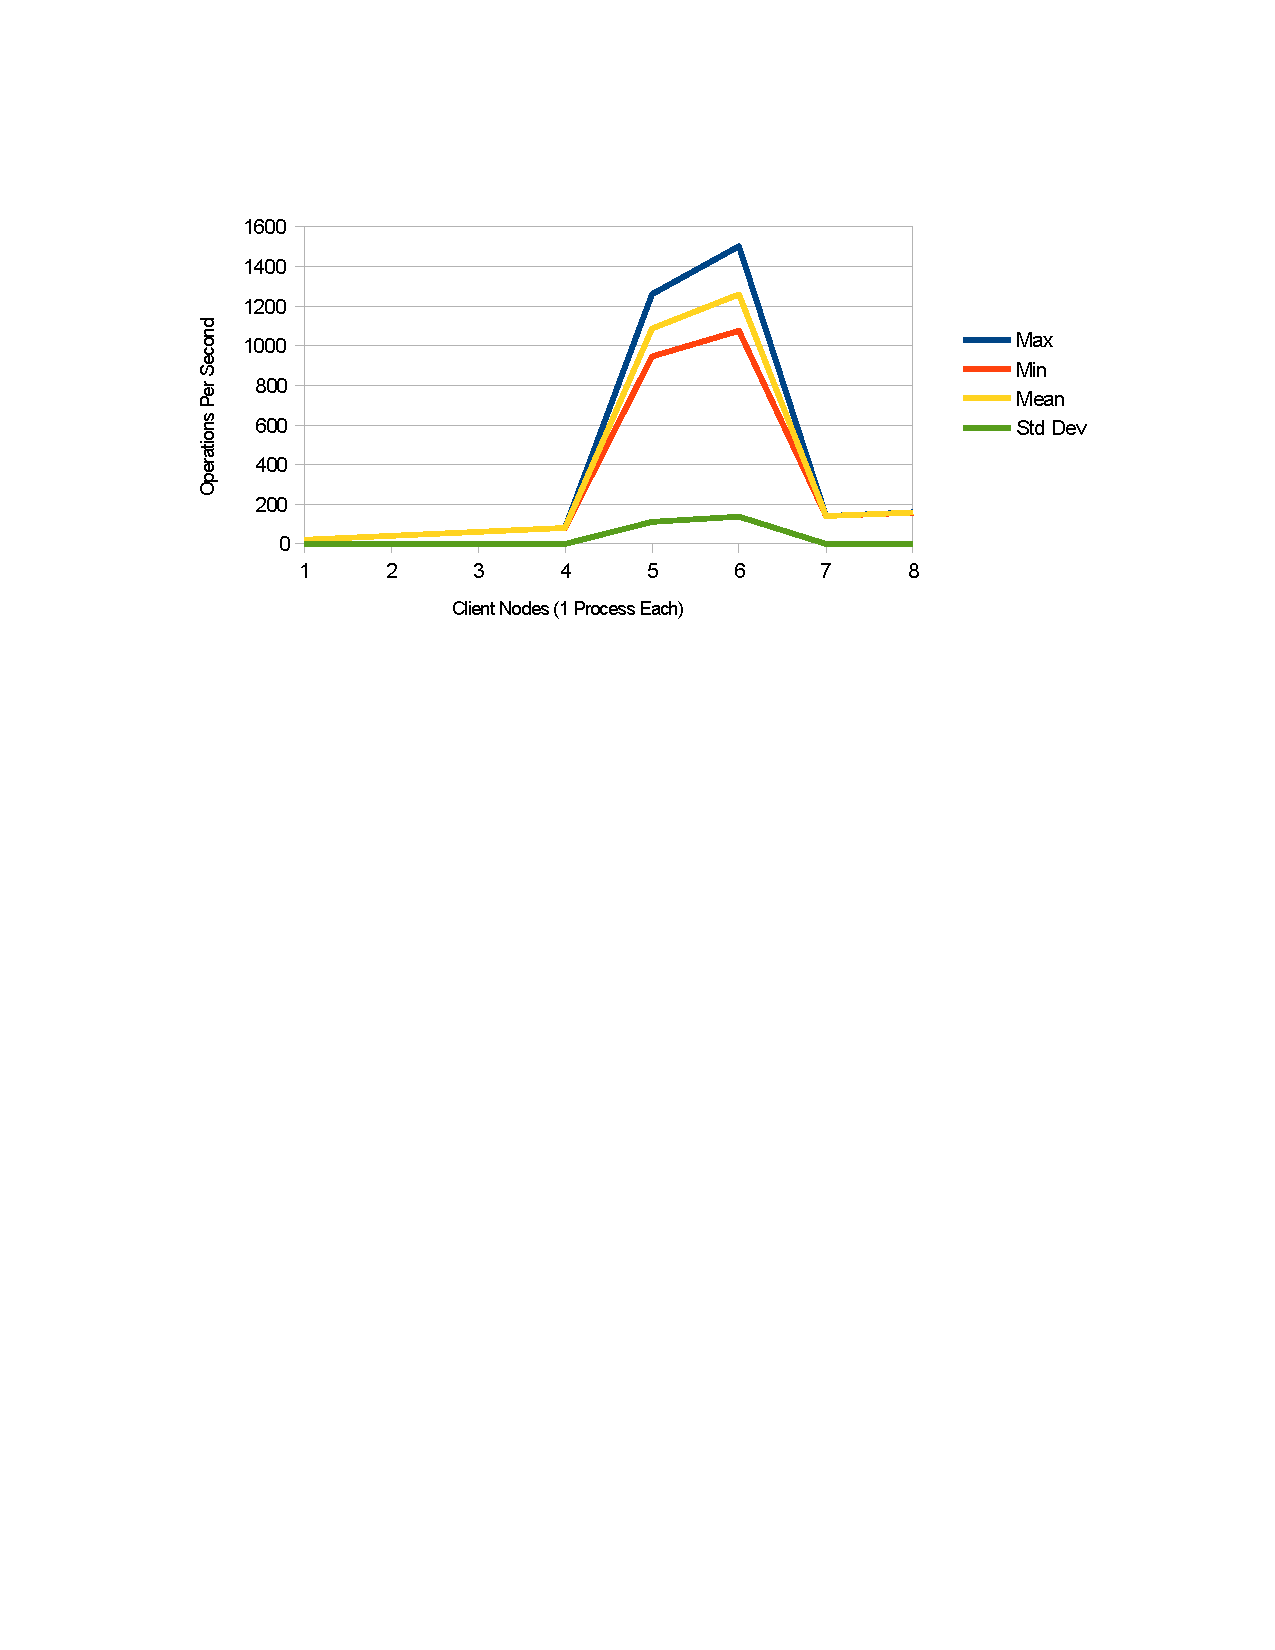
\includegraphics[width=3.5in]{mdtest-064-file-create}
\caption{mdtest of file creation on Ceph 0.64}
\label{fig:mdtest-064-file-create}
\end{figure}


The results also show that file creation rate is signficantly lower than
directory creation rate. We stipulated two contributing factors: one is the file
creation is associated with 1 MB data write and followed by a fsync operation,
which is a rather heavy weight operation compare to directory creation. Another
factor is that we obtained above results from early version of Ceph without all
the tunings and improvement applied. Therefore, we repeated the same test on the
latest CephFS 0.64. The result is illustrated in
Figure~\ref{fig:mdtest-064-file-create}. As expected, we observed a significant
improvement on the file creation rate. We also note that as number of clients
increase, the file creation rate decreases rapidly, which suggested some form of
lock contention. This presents some interesting issues to be investigated
further.


